% Name: Binary search
% Description: Binary search for 23 in a sorted array of ten numbers: each step compares the middle element and halves the range, finding 23 on the third step.
% Tags: binary search, sorted array, divide and conquer, algorithm

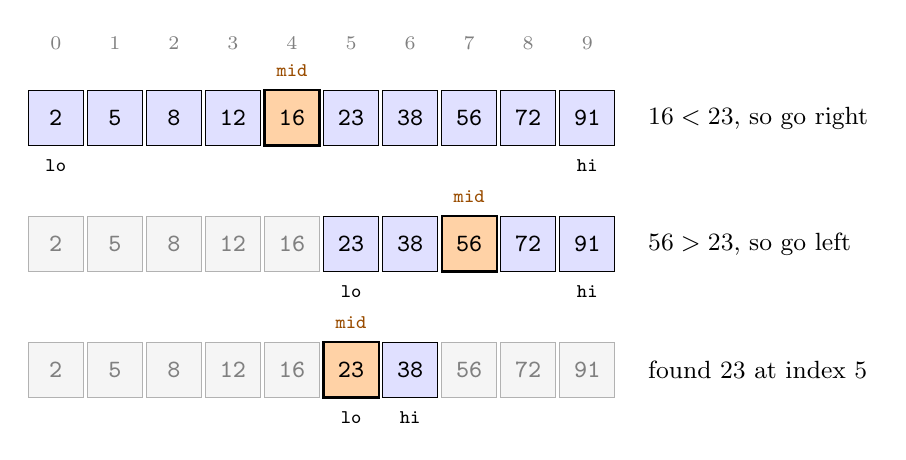
\begin{tikzpicture}[every node/.style={font=\small}]
  % Step s keeps indices lo..hi and checks mid = floor((lo + hi)/2): (0,9,4), then (5,9,7), then (5,6,5)
  \foreach \s/\lo/\hi/\mid/\note in {0/0/9/4/{$16 < 23$, so go right}, 1/5/9/7/{$56 > 23$, so go left}, 2/5/6/5/{found 23 at index 5}} {
    \pgfmathsetmacro\y{-1.6*\s}
    \foreach \v [count=\i from 0] in {2,5,8,12,16,23,38,56,72,91} {
      \pgfmathsetmacro\inrange{(\i >= \lo) && (\i <= \hi)}
      \ifnum\i=\mid
        \node[draw, thick, fill=orange!35, minimum size=7mm, font=\ttfamily\small] at (0.75*\i,\y) {\v};
      \else\ifdim\inrange pt>0pt
        \node[draw, fill=blue!12, minimum size=7mm, font=\ttfamily\small] at (0.75*\i,\y) {\v};
      \else
        \node[draw=gray!60, fill=gray!8, text=gray, minimum size=7mm, font=\ttfamily\small] at (0.75*\i,\y) {\v};
      \fi\fi
    }
    \node[font=\scriptsize\ttfamily, below=4mm] at (0.75*\lo,\y) {lo};
    \node[font=\scriptsize\ttfamily, below=4mm] at (0.75*\hi,\y) {hi};
    \node[font=\scriptsize\ttfamily, above=4mm, orange!60!black] at (0.75*\mid,\y) {mid};
    \node[anchor=west] at (7.4,\y) {\note};
  }
  \foreach \i in {0,...,9} \node[font=\scriptsize, gray] at (0.75*\i,0.95) {\i};
\end{tikzpicture}
